% Software Requirements Specification -- CampusGPT
% Build:  tectonic docs/srs/campus-gpt-srs.tex
\documentclass[11pt,a4paper,oneside]{report}

% ---------------------------------------------------------------------------
% Team details -- fill these in (placeholders are shown in red in the PDF)
% ---------------------------------------------------------------------------
\newcommand{\Fill}[1]{\textcolor{red}{[#1]}}
\newcommand{\MemberOne}{Ankur Karn & 500118986 & 11}
\newcommand{\MemberTwo}{Ashmita Sharma & 500122422 & 11}
\newcommand{\MemberThree}{Ananya Singh & 500123837 & 11}
\newcommand{\MemberFour}{Ayushi Mishra & 500121986 & 11}
\newcommand{\Specialization}{Cyber Security}
\newcommand{\Mentor}{Mr.~Yogesh Rathia}
\newcommand{\School}{School of Computer Science}
\newcommand{\University}{UNIVERSITY OF PETROLEUM \& ENERGY STUDIES}
\newcommand{\UniversityAddress}{Dehradun -- 248007, Uttarakhand}
\newcommand{\DocVersion}{1.0}

% ---------------------------------------------------------------------------
\usepackage[margin=2.5cm,headheight=14pt]{geometry}
\usepackage[T1]{fontenc}
\usepackage{lmodern}
\usepackage{microtype}
\usepackage{xcolor}
\usepackage{booktabs}
\usepackage{tabularx}
\usepackage{array}
\usepackage{longtable}
\usepackage{enumitem}
\usepackage{amsmath}
\usepackage{fancyhdr}
\usepackage{titlesec}
\usepackage{tikz}
\usetikzlibrary{positioning,arrows.meta,shapes.geometric}
\usepackage{pgfgantt}
\usepackage[most]{tcolorbox}
\usepackage{caption}
\usepackage{float}
\usepackage[hidelinks]{hyperref}
\usepackage{xurl}

\definecolor{algogreen}{HTML}{1F4D3A}
\captionsetup[table]{position=above,skip=4pt}
\setlength{\parindent}{0pt}
\setlength{\parskip}{6pt}
\renewcommand{\arraystretch}{1.15}
\newcolumntype{Y}{>{\raggedright\arraybackslash}X}

% Chapter headings: "CHAPTER 1" above the title, as in the sample
\titleformat{\chapter}[display]
  {\normalfont\bfseries}{\large\MakeUppercase{\chaptertitlename}~\thechapter}{4pt}{\Huge}
\titlespacing*{\chapter}{0pt}{0pt}{24pt}

% Header / footer
\pagestyle{fancy}
\fancyhf{}
\fancyhead[L]{\itshape SRS}
\fancyhead[R]{\itshape CampusGPT}
\fancyfoot[C]{Page \thepage}
\renewcommand{\headrulewidth}{0.4pt}
\fancypagestyle{plain}{%
  \fancyhf{}\fancyhead[L]{\itshape SRS}\fancyhead[R]{\itshape CampusGPT}%
  \fancyfoot[C]{Page \thepage}\renewcommand{\headrulewidth}{0.4pt}}

% Algorithm box
\newtcolorbox{algobox}[1]{enhanced,breakable,colback=white,colframe=algogreen,
  coltitle=white,fonttitle=\bfseries\sffamily,title={#1},arc=2mm,boxrule=0.6pt,
  left=6pt,right=6pt,top=4pt,bottom=4pt}

\begin{document}

% ===========================================================================
% Title page
% ===========================================================================
\hypersetup{pageanchor=false}
\begin{titlepage}
\thispagestyle{empty}
\centering
\vspace*{0.5cm}
{\Huge\bfseries Software Requirements\\[4pt] Specification\par}
\vspace{1.2cm}
{\LARGE\bfseries CampusGPT\par}
\vspace{0.3cm}
{\large\itshape An AI-Powered University Intelligence and Student Assistance Platform\par}
\vspace{1cm}
Submitted in partial fulfilment of the requirements for the award of the degree of\par
\vspace{0.3cm}
{\Large\bfseries Bachelor of Technology\par}
\vspace{0.15cm}
Computer Science and Engineering\par
Specialization: \textbf{\Specialization}\par
\vspace{1cm}
{\large\bfseries Prepared by\par}
\vspace{0.3cm}
\begin{tabular*}{0.8\textwidth}{@{\extracolsep{\fill}}lrr}
\toprule
\textbf{Name} & \textbf{SAP ID} & \textbf{Batch}\\
\midrule
\MemberOne\\
\MemberTwo\\
\MemberThree\\
\MemberFour\\
\bottomrule
\end{tabular*}\par
\vspace{1cm}
Under the guidance of\par
\vspace{0.15cm}
{\large\bfseries \Mentor\par}
\textit{Project Mentor}\par
\vfill
{\bfseries \School\par}
{\bfseries \University\par}
\UniversityAddress\par
\vspace{0.8cm}
{\large\bfseries October 2026 \quad$|$\quad Version \DocVersion\par}
\end{titlepage}
\hypersetup{pageanchor=true}

% ===========================================================================
% Front matter
% ===========================================================================
\pagenumbering{roman}
\setcounter{page}{1}
\tableofcontents
\listoffigures
\listoftables

\chapter*{Revision History}
\addcontentsline{toc}{chapter}{Revision History}
\begin{tabularx}{\textwidth}{|c|Y|Y|}
\hline
\textbf{Date} & \textbf{Change} & \textbf{Reason for Changes}\\
\hline
Tue, 13 Oct 2026 & Version 1.0. First complete draft: introduction, beneficiaries,
functional requirements, reference algorithms, SWOT analysis, PERT and Gantt schedule,
non-functional and security requirements, glossary, context diagram, and issues list. &
First submission for mentor review.\\
\hline
\end{tabularx}

\chapter*{Document Conventions}
\addcontentsline{toc}{chapter}{Document Conventions}
\begin{itemize}
  \item The document follows the structure recommended by IEEE Std
        830-1998~\cite{ieee830}.
  \item Requirements are written with \textbf{``shall''}. Each has an ID such as
        \textbf{FR-06} (functional), \textbf{NFR-P1} (non-functional, performance) or
        \textbf{NFR-S1} (non-functional, security) so it can be traced directly to design
        and testing.
  \item Priorities are \textbf{High} (needed for release), \textbf{Medium} (planned for
        release), and \textbf{Low} (good to have).
  \item Performance figures in Chapter~3 are \textbf{targets} to be verified during testing,
        not measured results.
  \item All student records and policy documents referred to in this document are
        \textbf{synthetic} (fictional) and are labelled as such inside the system.
\end{itemize}

% ===========================================================================
\clearpage
\pagenumbering{arabic}
\setcounter{page}{1}
\chapter{SRS Introduction}

\section{Purpose of the Project}
CampusGPT is an AI-powered helpdesk platform that gives university students a single
conversational interface to their academic and administrative information. Instead of
searching several portals, PDFs and notice boards, a student asks a question in natural
language, such as ``How many classes must I attend to reach 75\% in DBMS?''. The system
answers by combining two sources: the student's own records, fetched from a PostgreSQL
database through predefined, permission-checked backend tools, and university policy
documents, searched with Retrieval-Augmented Generation (RAG)~\cite{lewis2020rag} and cited
in the answer. The language model never queries the database directly, numerical results
are computed by deterministic code, and access to student data is enforced by the backend
rather than by prompt instructions. Because the project has no access to real university
systems, all data is synthetic, and the design permits a later switch to authorized
university APIs.

\section{Target Beneficiary}
Table~\ref{tab:beneficiaries} delineates target user groups and direct benefits.

\begin{table}[H]
\centering
\caption{Target beneficiaries and the benefit to each}
\label{tab:beneficiaries}
\begin{tabularx}{\textwidth}{@{}>{\bfseries\raggedright\arraybackslash}p{3.6cm}YY@{}}
\toprule
\textnormal{\textbf{Beneficiary}} & \textbf{Who they are} & \textbf{How CampusGPT helps}\\
\midrule
Students & Undergraduate students enrolled in university programs &
Instant answers about their attendance, exams, assignments, fees and the rules that apply,
with sources shown; a prioritised weekly summary.\\
University Administrators & Academic office and helpdesk staff &
Fewer repetitive queries; policy documents and notices published once and immediately
answerable in chat.\\
Faculty Advisors & Teachers mentoring student groups &
Students arrive with accurate, policy-backed information (direct faculty access is planned
for a later version).\\
University IT Department & Teams maintaining ERP and portal systems &
A conversational layer that connects to existing systems through a defined adapter,
without replacing them.\\
\bottomrule
\end{tabularx}
\end{table}

\section{Functional Requirements}
The functional requirements of CampusGPT are cataloged in Table~\ref{tab:fr}.

\begin{longtable}{@{}>{\raggedright\arraybackslash}p{1.5cm}>{\raggedright\arraybackslash}p{3.4cm}>{\raggedright\arraybackslash}p{1.7cm}>{\raggedright\arraybackslash}p{7.4cm}@{}}
\caption{Functional requirements of CampusGPT}\label{tab:fr}\\
\toprule
\textbf{ID} & \textbf{Requirement Name} & \textbf{Priority} & \textbf{The system shall\ldots}\\
\midrule
\endfirsthead
\toprule
\textbf{ID} & \textbf{Requirement Name} & \textbf{Priority} & \textbf{The system shall\ldots}\\
\midrule
\endhead
\bottomrule
\endfoot
\textbf{FR-01} & Synthetic Data Generation & High & Generate a reproducible (seeded) synthetic
university of 3,000--5,000 students with consistent programs, courses, enrollments,
attendance, exams, assignments and fees.\\
\textbf{FR-02} & Synthetic Labelling & High & Label every generated record and policy
document as synthetic demonstration data.\\
\textbf{FR-03} & Authentication & High & Authenticate users by email and password, storing
passwords as Argon2id hashes~\cite{biryukov2016argon2}.\\
\textbf{FR-04} & Role-Based Access & High & Support \emph{student} and \emph{administrator}
roles and restrict every endpoint by role~\cite{sandhu1996rbac}.\\
\textbf{FR-05} & Student Data Isolation & High & Derive the student identity for every data
request from the authenticated session, never from user or model input.\\
\textbf{FR-06} & Student Dashboard & High & Display the logged-in student's attendance,
upcoming exams, pending assignments and fee status.\\
\textbf{FR-07} & Conversational Chat & High & Accept natural-language questions and keep
per-user conversation history.\\
\textbf{FR-08} & Tool Calling & High & Answer student-specific questions only through
predefined, read-only backend tools; the model shall not generate or execute SQL.\\
\textbf{FR-09} & Attendance Calculator & High & Compute classes required to reach, or
classes that may be missed while staying above, an attendance threshold using
deterministic code.\\
\textbf{FR-10} & Document Ingestion & High & Extract, clean, chunk and embed policy
documents (PDF or text) and store the vectors in PostgreSQL with pgvector.\\
\textbf{FR-11} & Hybrid Retrieval & Medium & Retrieve relevant chunks by combining vector
similarity and keyword search using Reciprocal Rank Fusion~\cite{cormack2009rrf}.\\
\textbf{FR-12} & Source Citations & High & Cite, in every policy-based answer, the
document and section of each chunk actually used, and mark database-derived facts as such.\\
\textbf{FR-13} & Weekly Summary & High & Produce a prioritised list of items needing the
student's attention in the next seven days.\\
\textbf{FR-14} & Admin Document Upload & Medium & Allow administrators to upload, replace
and delete policy documents and notices, re-indexing them automatically.\\
\textbf{FR-15} & Audit Logging & Medium & Record logins, tool executions and administrative
actions with user, time and outcome, excluding sensitive field values.\\
\textbf{FR-16} & AI Outage Fallback & Medium & Keep the dashboard and all non-chat pages
working, and show a clear message in chat, when the language-model service is unavailable.\\
\textbf{FR-17} & Suggested Questions & Low & Offer example questions to new users in the
chat interface.\\
\end{longtable}

% ===========================================================================
\chapter{SRS Project Description}

\section{Reference Algorithms and Concepts}
CampusGPT maps student questions to verified data sources and methods
(Table~\ref{tab:methods}). The orchestration follows the tool-use pattern of
ReAct~\cite{yao2023react} and Toolformer~\cite{schick2023toolformer}, restricted to a fixed
tool catalogue.

\begin{table}[H]
\centering
\caption{Student questions and the method used to answer each}
\label{tab:methods}
\begin{tabularx}{\textwidth}{@{}YY>{\raggedright\arraybackslash}p{3.2cm}@{}}
\toprule
\textbf{Student Question} & \textbf{Computational Method} & \textbf{Used in}\\
\midrule
What is my attendance in DBMS? & Session-scoped tool \texttt{get\_my\_attendance} (SQL
inside the backend) & Chat, Dashboard\\
How many classes must I attend to reach 75\%? & Deterministic formula (Algorithm~3) &
Attendance calculator tool, Chat\\
What is the attendance rule for exams? & Hybrid RAG: pgvector HNSW~\cite{malkov2020hnsw}
search + full-text search, fused by RRF & Chat (with citations)\\
Can I sit for my exam? & Tool result + retrieved policy, combined by the LLM & Chat\\
What do I need to take care of this week? & Rule-based urgency scoring, explained by the
LLM & Weekly Summary\\
\bottomrule
\end{tabularx}
\end{table}

\begin{algobox}{Algorithm 1: Policy Document Ingestion and Indexing}
\begin{enumerate}[leftmargin=*,itemsep=1pt]
  \item Validate the upload (administrator role, PDF/TXT type, size $\le$ 10\,MB).
  \item Extract text page by page; remove headers, footers and repeated whitespace.
  \item Split into chunks of about 500 tokens with 50-token overlap, keeping the document
        title, section heading and page number as metadata.
  \item Embed each chunk with a local open-source embedding model
        (BGE-small~\cite{xiao2024cpack}, 384 dimensions) on the CPU.
  \item Store chunks, metadata and vectors in PostgreSQL; build the HNSW vector index and
        the full-text index.
  \item Mark the previous version of the same document as superseded so that only the
        current version is retrieved.
\end{enumerate}
\end{algobox}

\begin{algobox}{Algorithm 2: Authenticated Question Answering with Tools and Citations}
\begin{enumerate}[leftmargin=*,itemsep=1pt]
  \item Authenticate the request from the session cookie; load \texttt{user\_id} and role.
  \item Send the question, conversation history and the tool list permitted for the role to
        the LLM through the provider adapter.
  \item For each tool call requested by the LLM: check the tool is in the role's allow-list,
        validate its arguments against the tool's schema, inject \texttt{student\_id} from
        the session, execute it, and write an audit-log entry.
  \item Return tool results and retrieved policy chunks (each with a chunk ID) to the LLM,
        wrapped as untrusted data~\cite{greshake2023injection}.
  \item Receive the final answer; verify that every cited chunk ID was actually retrieved and
        drop any citation that was not.
  \item Return the answer with its database and document sources; store the turn in the
        conversation history.
\end{enumerate}
\end{algobox}

\begin{algobox}{Algorithm 3: Attendance Requirement Calculation}
\begin{enumerate}[leftmargin=*,itemsep=1pt]
  \item Read attended classes $a$ and total classes held $t$ for the course; read threshold
        $p$ (e.g.\ $0.75$) from configuration.
  \item If $a/t < p$: classes needed $x = \left\lceil \dfrac{p\,t - a}{1 - p} \right\rceil$,
        the smallest $x$ with $(a+x)/(t+x) \ge p$.
  \item Else: classes that may be missed
        $m = \left\lfloor \dfrac{a - p\,t}{p} \right\rfloor$, the largest $m$ with
        $a/(t+m) \ge p$.
  \item Return $a$, $t$, current percentage, and $x$ or $m$, labelled as a calculated value.
\end{enumerate}
\end{algobox}

\clearpage
\section{SWOT Analysis}
Table~\ref{tab:swot} presents the SWOT analysis of the CampusGPT platform.

\begin{table}[H]
\centering
\caption{SWOT analysis of CampusGPT}
\label{tab:swot}
\begin{tabularx}{\textwidth}{@{}Y|Y@{}}
\toprule
\textbf{STRENGTHS (Internal)} & \textbf{WEAKNESSES (Internal)}\\
\midrule
$\bullet$ Answers grounded in database records and cited policy text.\newline
$\bullet$ Student data isolation enforced in the backend, not by prompts.\newline
$\bullet$ Deterministic calculations for attendance and deadlines.\newline
$\bullet$ Fully free stack: open-source software, local embeddings, free-tier LLM API.\newline
$\bullet$ Swappable LLM provider through a single adapter. &
$\bullet$ Uses synthetic data only; no live university integration.\newline
$\bullet$ Free-tier LLM APIs impose rate limits.\newline
$\bullet$ English only in the first version.\newline
$\bullet$ Scanned (image-only) PDFs are not supported.\newline
$\bullet$ Smaller models may select the wrong tool for complex questions.\\
\midrule
\textbf{OPPORTUNITIES (External)} & \textbf{THREATS (External)}\\
\midrule
$\bullet$ Integration with university ERP systems through authorized APIs.\newline
$\bullet$ Multilingual support through Indian-language speech and translation models.\newline
$\bullet$ Extension to faculty and administrative staff.\newline
$\bullet$ Delivery through mobile apps or messaging platforms. &
$\bullet$ Changes in free-tier limits or terms of LLM providers.\newline
$\bullet$ New prompt-injection techniques~\cite{owasp2025llm}.\newline
$\bullet$ Compliance obligations under the DPDP Act, 2023~\cite{dpdp2023} for real
deployments.\newline
$\bullet$ Loss of student trust after an incorrect answer~\cite{ji2023hallucination}.\\
\bottomrule
\end{tabularx}
\end{table}

\section{Project Schedule, PERT and Gantt Analysis}
The engineering lifecycle is executed over 31 days (13 October to 12 November 2026),
developed iteratively~\cite{larman2003iterative}. Table~\ref{tab:pert} documents the
activity network, with durations in days. Activities with zero slack form the Critical
Path: \textbf{A $\rightarrow$ B $\rightarrow$ D $\rightarrow$ E $\rightarrow$ G
$\rightarrow$ H $\rightarrow$ J $\rightarrow$ M $\rightarrow$ N} (Total: 31 days).
Figure~\ref{fig:gantt} shows the corresponding Gantt chart.

\begin{table}[H]
\centering
\caption{PERT activity table (durations in days)}
\label{tab:pert}
\small
\begin{tabular}{@{}clcccccc@{}}
\toprule
\textbf{ID} & \textbf{Activity Description} & \textbf{Dur.} & \textbf{Pred.} &
\textbf{ES} & \textbf{EF} & \textbf{LS} & \textbf{Slack}\\
\midrule
A & Problem study \& requirements (SRS)      & 2 & --      & 0  & 2  & 0  & \textbf{0}\\
B & Literature review \& toolchain setup      & 2 & A       & 2  & 4  & 2  & \textbf{0}\\
C & Synthetic policy documents               & 5 & A       & 2  & 7  & 11 & 9\\
D & Database schema \& migrations             & 3 & B       & 4  & 7  & 4  & \textbf{0}\\
E & Synthetic data generator                 & 4 & D       & 7  & 11 & 7  & \textbf{0}\\
F & Authentication \& RBAC                    & 3 & D       & 7  & 10 & 8  & 1\\
G & Student APIs \& dashboard                 & 5 & E, F    & 11 & 16 & 11 & \textbf{0}\\
H & LLM adapter \& tool calling               & 5 & G       & 16 & 21 & 16 & \textbf{0}\\
I & RAG ingestion, retrieval \& citations     & 5 & C, D    & 7  & 12 & 16 & 9\\
J & Weekly summary (Campus Intelligence)     & 3 & H, I    & 21 & 24 & 21 & \textbf{0}\\
K & Admin document upload                    & 2 & I       & 12 & 14 & 22 & 10\\
L & Evaluation benchmark questions           & 5 & C       & 7  & 12 & 19 & 12\\
M & Security testing \& evaluation            & 4 & J, K, L & 24 & 28 & 24 & \textbf{0}\\
N & Report, demonstration \& defense          & 3 & M       & 28 & 31 & 28 & \textbf{0}\\
\bottomrule
\end{tabular}
\end{table}

\begin{figure}[H]
\centering
\resizebox{\textwidth}{!}{%
\begin{ganttchart}[
    hgrid, vgrid={dotted},
    time slot format=isodate,
    x unit=0.42cm, y unit chart=0.55cm,
    title height=1,
    title label font=\scriptsize,
    bar/.append style={fill=algogreen!25, draw=algogreen},
    bar label font=\small,
    milestone/.append style={fill=red!70},
    link/.style={-latex, draw=gray}
  ]{2026-10-13}{2026-11-12}
  \gantttitlecalendar{month=name, day} \\
  \ganttbar{A Requirements}{2026-10-13}{2026-10-14} \\
  \ganttbar{B Toolchain}{2026-10-15}{2026-10-16} \\
  \ganttbar{C Policy documents}{2026-10-15}{2026-10-19} \\
  \ganttbar{D Database schema}{2026-10-17}{2026-10-19} \\
  \ganttbar{E Data generator}{2026-10-20}{2026-10-23} \\
  \ganttbar{F Auth \& RBAC}{2026-10-20}{2026-10-22} \\
  \ganttbar{G APIs \& dashboard}{2026-10-24}{2026-10-28} \\
  \ganttbar{H LLM \& tools}{2026-10-29}{2026-11-02} \\
  \ganttbar{I RAG \& citations}{2026-10-20}{2026-10-24} \\
  \ganttbar{J Weekly summary}{2026-11-03}{2026-11-05} \\
  \ganttbar{K Admin upload}{2026-10-25}{2026-10-26} \\
  \ganttbar{L Benchmark}{2026-10-20}{2026-10-24} \\
  \ganttbar{M Testing \& eval.}{2026-11-06}{2026-11-09} \\
  \ganttbar{N Report \& defense}{2026-11-10}{2026-11-12} \\
  \ganttmilestone{Submission}{2026-11-12}
\end{ganttchart}}
\caption{Gantt chart of the CampusGPT schedule (13 Oct -- 12 Nov 2026).}
\label{fig:gantt}
\end{figure}

% ===========================================================================
\chapter{SRS Non-Functional Requirements}

\section{Performance Requirements}
Table~\ref{tab:perf} itemizes the performance targets of CampusGPT. They are measured
on the development machine (Intel Core i5-12450HX, 8\,GB RAM) with the full synthetic
dataset loaded.

\begin{table}[H]
\centering
\caption{Performance requirements of CampusGPT}
\label{tab:perf}
\begin{tabularx}{\textwidth}{@{}lYc@{}}
\toprule
\textbf{ID} & \textbf{Requirement Statement} & \textbf{Measurable Target}\\
\midrule
NFR-P1 & Dashboard API response time & $<$ 300 ms (95th percentile)\\
NFR-P2 & Single tool execution (database query) & $<$ 100 ms (95th percentile)\\
NFR-P3 & Hybrid document retrieval & $<$ 500 ms per query\\
NFR-P4 & End-to-end chat answer, hosted LLM & $<$ 8 s median\\
NFR-P5 & Synthetic data generation, 5,000 students & $<$ 5 min\\
NFR-P6 & Ingestion of a 20-page policy PDF & $<$ 60 s on CPU\\
NFR-P7 & Backend memory incl.\ embedding model & $<$ 1.5 GB resident\\
NFR-P8 & Automated test suite execution & $<$ 2 min\\
\bottomrule
\end{tabularx}
\end{table}

\section{Security Requirements}
Table~\ref{tab:sec} lists the security requirements, derived from the OWASP Top
10~\cite{owasp2021} and the OWASP Top 10 for LLM Applications~\cite{owasp2025llm}.

\begin{table}[H]
\centering
\caption{Security requirements of CampusGPT}
\label{tab:sec}
\begin{tabularx}{\textwidth}{@{}lY@{}}
\toprule
\textbf{ID} & \textbf{The system shall\ldots}\\
\midrule
NFR-S1 & Return zero records belonging to another student in all cross-user access tests,
whether attempted through the API, by changing IDs in the browser, or through prompts.\\
NFR-S2 & Reject any tool call outside the caller's role allow-list, regardless of the LLM's
request.\\
NFR-S3 & Treat uploaded document text as untrusted data and never as instructions.\\
NFR-S4 & Store secrets only in environment variables, never in the source repository.\\
NFR-S5 & Rate-limit login and chat endpoints per user and per IP address.\\
NFR-S6 & Exclude passwords, tokens and personal fields from application logs.\\
\bottomrule
\end{tabularx}
\end{table}

\section{Software Quality Attributes (ISO/IEC 25010)}
Table~\ref{tab:quality} maps system quality characteristics to the ISO/IEC 25010
standard~\cite{iso25010}.

\begin{table}[H]
\centering
\caption{Software quality attributes mapped to ISO/IEC 25010}
\label{tab:quality}
\begin{tabularx}{\textwidth}{@{}>{\bfseries\raggedright\arraybackslash}p{3.8cm}Y@{}}
\toprule
\textnormal{\textbf{Quality Attribute}} & \textbf{How CampusGPT Achieves It}\\
\midrule
Functional Suitability & Answers student questions from database records and cited policy
text; correctness measured on a benchmark question set~\cite{es2024ragas}.\\
Performance Efficiency & Indexed queries, HNSW vector index, local CPU embeddings, and
bounded context size.\\
Compatibility & REST API documented with OpenAPI~\cite{fastapi}; LLM provider and
university data source isolated behind adapters.\\
Interaction Capability & Single chat interface with suggested questions, readable formatting
and visible sources; responsive dashboard~\cite{nextjs}.\\
Reliability & Non-chat features keep working during LLM outages; clear error messages on
tool failure.\\
Security & Session authentication, role-based access, server-side data isolation, audit
logs, and input validation.\\
Maintainability & Modular separation of API, tools, retrieval and provider adapter, with an
automated test suite.\\
Flexibility & Runs on Linux, macOS and Windows; PostgreSQL~\cite{postgresql} and
pgvector~\cite{pgvector} run locally or on a hosted service.\\
\bottomrule
\end{tabularx}
\end{table}

% ===========================================================================
\appendix
\chapter{Glossary}

\begin{longtable}{@{}>{\bfseries\raggedright\arraybackslash}p{3.6cm}>{\raggedright\arraybackslash}p{11cm}@{}}
\caption{Glossary of terms and abbreviations}\label{tab:glossary}\\
\toprule
\textnormal{\textbf{Term}} & \textbf{Definition}\\
\midrule
\endfirsthead
\toprule
\textnormal{\textbf{Term}} & \textbf{Definition}\\
\midrule
\endhead
\bottomrule
\endfoot
LLM & Large Language Model: a neural network that generates text from a prompt.\\
RAG & Retrieval-Augmented Generation: supplying retrieved documents to an LLM so its answer
is based on them.\\
Embedding & A fixed-length numeric vector representing the meaning of a piece of text.\\
Chunk & A short section of a document that is embedded and retrieved as one unit.\\
pgvector & A PostgreSQL extension for storing vectors and running similarity search.\\
HNSW & Hierarchical Navigable Small World: a graph-based index for fast approximate
nearest-neighbour search.\\
Hybrid Search & Retrieval combining vector similarity with keyword (full-text) matching.\\
RRF & Reciprocal Rank Fusion: a method for merging several ranked result lists into one.\\
Tool Calling & An LLM requesting that the application run a named function with given
arguments.\\
Prompt Injection & Text crafted to make an LLM ignore its instructions or misuse its tools.\\
Hallucination & LLM output that is fluent but not supported by the provided sources.\\
RBAC & Role-Based Access Control: permissions granted according to a user's role.\\
Argon2id & A memory-hard password-hashing algorithm.\\
Synthetic Data & Artificially generated records that resemble real data but describe no real
person.\\
DPDP Act & India's Digital Personal Data Protection Act, 2023.\\
\end{longtable}

\chapter{Analysis Model}

\begin{figure}[H]
\centering
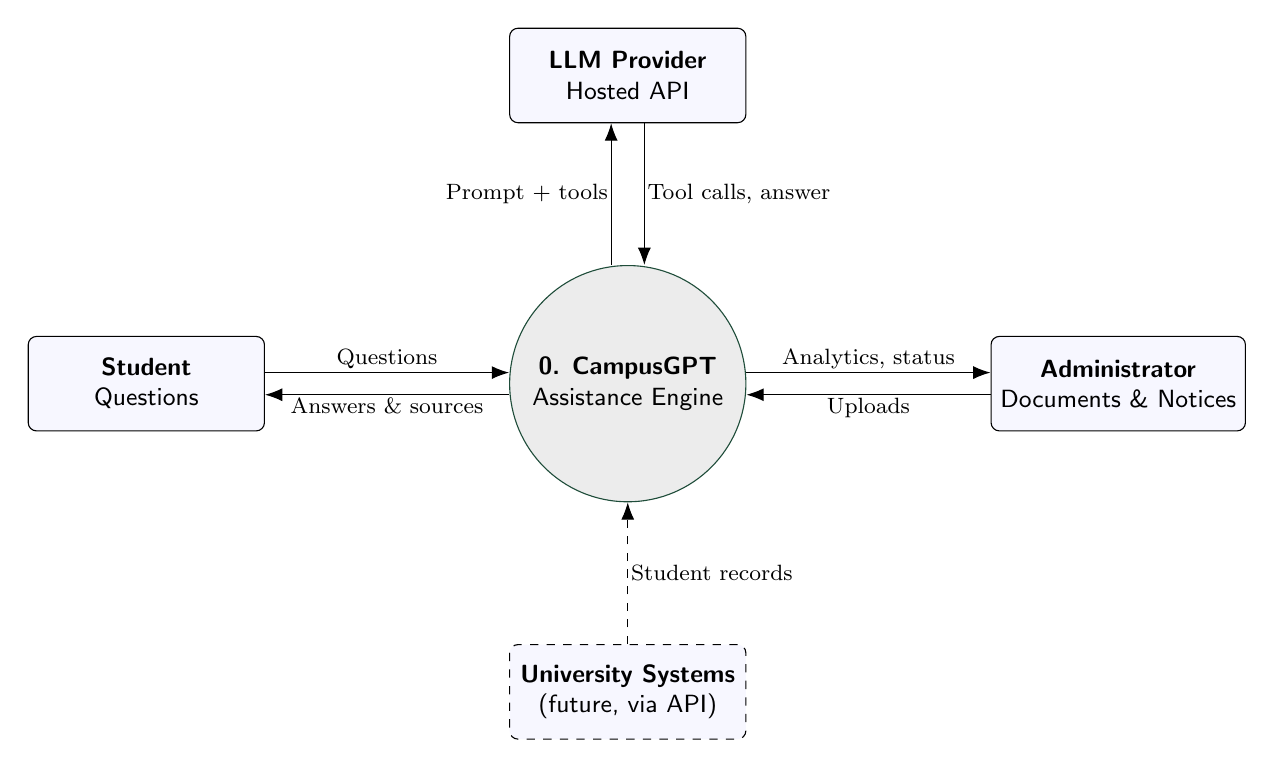
\begin{tikzpicture}[
  ent/.style={draw, rounded corners=3pt, fill=blue!3, align=center, minimum width=3cm,
              minimum height=1.2cm, font=\sffamily\small},
  proc/.style={circle, draw=algogreen, fill=gray!15, align=center, minimum size=3cm,
               font=\sffamily\small},
  lab/.style={font=\footnotesize, fill=white, inner sep=1pt},
  >={Latex[length=2.2mm]}]
  \node[proc] (sys) {\textbf{0. CampusGPT}\\Assistance Engine};
  \node[ent, left=3.1cm of sys] (stu) {\textbf{Student}\\Questions};
  \node[ent, right=3.1cm of sys] (adm) {\textbf{Administrator}\\Documents \& Notices};
  \node[ent, above=1.8cm of sys] (llm) {\textbf{LLM Provider}\\Hosted API};
  \node[ent, below=1.8cm of sys, dashed] (erp) {\textbf{University Systems}\\(future, via API)};
  \draw[->] ([yshift=4pt]stu.east) -- node[lab, above] {Questions} ([yshift=4pt]sys.west|-stu.east);
  \draw[<-] ([yshift=-4pt]stu.east) -- node[lab, below] {Answers \& sources} ([yshift=-4pt]sys.west|-stu.east);
  \draw[<-] ([yshift=4pt]adm.west) -- node[lab, above] {Analytics, status} ([yshift=4pt]sys.east|-adm.west);
  \draw[->] ([yshift=-4pt]adm.west) -- node[lab, below] {Uploads} ([yshift=-4pt]sys.east|-adm.west);
  \draw[->] ([xshift=-6pt]sys.north) -- node[lab, left] {Prompt + tools} ([xshift=-6pt]llm.south);
  \draw[<-] ([xshift=6pt]sys.north) -- node[lab, right] {Tool calls, answer} ([xshift=6pt]llm.south);
  \draw[->, dashed] (erp) -- node[lab, right] {Student records} (sys);
\end{tikzpicture}
\caption{Level-0 Context Diagram of CampusGPT.}
\label{fig:context}
\end{figure}

Figure~\ref{fig:context} shows CampusGPT as a single process. Students send questions and
receive answers with sources; administrators upload documents and notices; the hosted LLM
receives only the prompt, permitted tool definitions and retrieved context. In the current
version, student records come from the synthetic PostgreSQL database; the dashed University
Systems entity marks the planned integration point.

\chapter{Issues List}

\begin{table}[H]
\centering
\caption{Living register of engineering issues and roadmap resolutions}
\label{tab:issues}
\begin{tabularx}{\textwidth}{@{}lYcY@{}}
\toprule
\textbf{ID} & \textbf{Description of Engineering Issue} & \textbf{Status} &
\textbf{Planned Resolution}\\
\midrule
I-01 & No authorized access to real university data; all records are synthetic. & Open &
Implement a university-API adapter behind the existing tool interface.\\
I-02 & Free-tier LLM APIs impose request rate limits. & Open & Cache repeated answers;
fall back to a local model.\\
I-03 & Scanned (image-only) PDFs cannot be ingested. & Deferred & Add an OCR step to the
ingestion pipeline.\\
I-04 & Interface and answers are English only. & Deferred & Integrate Indian-language
translation and speech models.\\
I-05 & Faculty role is not implemented. & Deferred & Add faculty role with course-scoped
tools.\\
I-06 & All tools are read-only; students cannot submit requests. & Deferred & Add
confirmation-gated write tools (e.g.\ hostel leave) with audit logging.\\
\bottomrule
\end{tabularx}
\end{table}

% ===========================================================================
\renewcommand{\bibname}{References}
\begin{thebibliography}{99}
\addcontentsline{toc}{chapter}{References}

\bibitem{ieee830}
IEEE, \emph{IEEE Recommended Practice for Software Requirements Specifications}, IEEE Std
830-1998, 1998.

\bibitem{lewis2020rag}
P.~Lewis \emph{et al.}, ``Retrieval-augmented generation for knowledge-intensive NLP
tasks,'' in \emph{Advances in Neural Information Processing Systems (NeurIPS 33)}, 2020,
pp.~9459--9474.

\bibitem{biryukov2016argon2}
A.~Biryukov, D.~Dinu, and D.~Khovratovich, ``Argon2: New generation of memory-hard functions
for password hashing and other applications,'' in \emph{Proc. IEEE European Symposium on
Security and Privacy (EuroS\&P)}, 2016, pp.~292--302.

\bibitem{sandhu1996rbac}
R.~S. Sandhu, E.~J. Coyne, H.~L. Feinstein, and C.~E. Youman, ``Role-based access control
models,'' \emph{Computer}, vol.~29, no.~2, pp.~38--47, 1996.

\bibitem{cormack2009rrf}
G.~V. Cormack, C.~L.~A. Clarke, and S.~Buettcher, ``Reciprocal rank fusion outperforms
Condorcet and individual rank learning methods,'' in \emph{Proc. 32nd ACM SIGIR}, 2009,
pp.~758--759.

\bibitem{yao2023react}
S.~Yao \emph{et al.}, ``ReAct: Synergizing reasoning and acting in language models,'' in
\emph{Proc. International Conference on Learning Representations (ICLR)}, 2023.

\bibitem{schick2023toolformer}
T.~Schick \emph{et al.}, ``Toolformer: Language models can teach themselves to use tools,''
in \emph{Advances in Neural Information Processing Systems (NeurIPS 36)}, 2023.

\bibitem{malkov2020hnsw}
Y.~A. Malkov and D.~A. Yashunin, ``Efficient and robust approximate nearest neighbor search
using hierarchical navigable small world graphs,'' \emph{IEEE Trans. Pattern Analysis and
Machine Intelligence}, vol.~42, no.~4, pp.~824--836, 2020.

\bibitem{xiao2024cpack}
S.~Xiao \emph{et al.}, ``C-Pack: Packed resources for general Chinese embeddings,'' in
\emph{Proc. 47th ACM SIGIR}, 2024, pp.~641--649.

\bibitem{greshake2023injection}
K.~Greshake \emph{et al.}, ``Not what you've signed up for: Compromising real-world
LLM-integrated applications with indirect prompt injection,'' in \emph{Proc. 16th ACM
Workshop on Artificial Intelligence and Security (AISec)}, 2023, pp.~79--90.

\bibitem{owasp2025llm}
OWASP Foundation, ``OWASP Top 10 for Large Language Model Applications,'' 2025. [Online].
Available: \url{https://genai.owasp.org/llm-top-10/}

\bibitem{dpdp2023}
Government of India, \emph{The Digital Personal Data Protection Act, 2023 (Act No.~22 of
2023)}, New Delhi, 2023.

\bibitem{ji2023hallucination}
Z.~Ji \emph{et al.}, ``Survey of hallucination in natural language generation,''
\emph{ACM Computing Surveys}, vol.~55, no.~12, Art.~248, 2023.

\bibitem{larman2003iterative}
C.~Larman and V.~R. Basili, ``Iterative and incremental development: A brief history,''
\emph{Computer}, vol.~36, no.~6, pp.~47--56, 2003.

\bibitem{owasp2021}
OWASP Foundation, ``OWASP Top 10:2021 Web Application Security Risks,'' 2021. [Online].
Available: \url{https://owasp.org/Top10/}

\bibitem{iso25010}
ISO/IEC, \emph{Systems and Software Engineering -- Systems and Software Quality Requirements
and Evaluation (SQuaRE) -- Product Quality Model}, ISO/IEC 25010:2023, 2023.

\bibitem{es2024ragas}
S.~Es, J.~James, L.~Espinosa-Anke, and S.~Schockaert, ``RAGAS: Automated evaluation of
retrieval augmented generation,'' in \emph{Proc. 18th Conf. European Chapter of the ACL:
System Demonstrations}, 2024, pp.~150--158.

\bibitem{fastapi}
S.~Ram\'irez, ``FastAPI documentation,'' 2024. [Online]. Available:
\url{https://fastapi.tiangolo.com/}

\bibitem{nextjs}
Vercel, ``Next.js documentation,'' 2024. [Online]. Available: \url{https://nextjs.org/docs}

\bibitem{postgresql}
The PostgreSQL Global Development Group, ``PostgreSQL documentation,'' 2024. [Online].
Available: \url{https://www.postgresql.org/docs/}

\bibitem{pgvector}
A.~Kane, ``pgvector: Open-source vector similarity search for Postgres,'' 2024. [Online].
Available: \url{https://github.com/pgvector/pgvector}

\end{thebibliography}

\end{document}
